
%ME20B183 BEGINNING POINT
\section{Swapnil Paresh Mehta}
\subsection{Clausius Theorem}
The Clausius theorem (1855) states that for a thermodynamic system (e.g. heat engine or heat pump) exchanging heat with external reservoirs and undergoing a thermodynamic cycle,
\linebreak
\begin{center}

\begin{equation}

   \oint \dfrac{\delta Q}{T_{Surr}} \leqslant 0
\label{eqn:CLAUSIUS}
\end{equation}

\end{center}
\begin{itemize}
\item $\delta Q$ - The infinitesimal amount of heat absorbed by the system from the reservoir
\item $T_{Surr}$ - The temperature of the external reservoir (surroundings) at a particular instant in time.
\end{itemize}

\subsection{Importance}
The Clausius theorem ~\ref{eqn:CLAUSIUS} is a mathematical explanation of the second law of thermodynamics. It was developed by Rudolf Clausius who intended to explain the relationship between the heat flow in a system and the entropy of the system and its surroundings. Clausius developed this in his efforts to explain entropy and define it quantitatively. In more direct terms, the theorem gives us a way to determine if a cyclical process is reversible or irreversible. The Clausius theorem provides a quantitative formula for understanding the second law.

\begin{figure}[hbtp]
\caption{Carnot Engine}
\centering
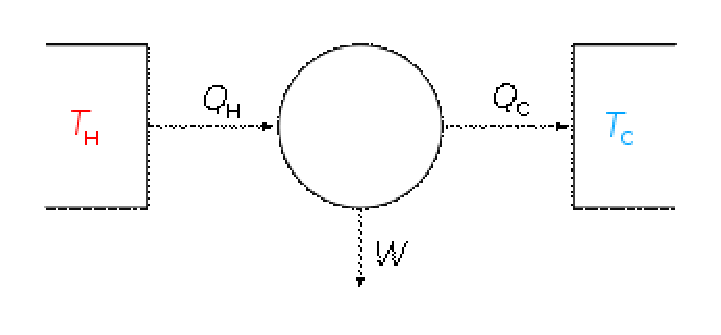
\includegraphics[]{ME20B183.eps}
\label{fig:CARNOT}
\end{figure}



\pagebreak
The above figure ~\ref{fig:CARNOT} is a figure for the classical Carnot Engine.
\subsection{References}
~\cite{webref}
